\documentclass[11pt,a4paper]{article}

\usepackage[a4paper,margin=2.25cm]{geometry}
\usepackage{graphicx}
\usepackage{subcaption}
\usepackage{booktabs}
\usepackage{tabularx}
\usepackage{array}
\usepackage{float}
\usepackage{xcolor}
\usepackage{hyperref}
\usepackage{enumitem}
\usepackage{microtype}

\definecolor{uantwerpred}{HTML}{C0002B}

\hypersetup{
  colorlinks=true,
  linkcolor=uantwerpred,
  citecolor=uantwerpred,
  urlcolor=uantwerpred
}

\graphicspath{{outputs/figures/}{outputs/figures/retrieval/}}
\setlength{\parskip}{0.42em}
\setlength{\parindent}{0pt}
\renewcommand{\arraystretch}{1.12}

\newcommand{\model}[1]{\texttt{#1}}
\newcommand{\githuburl}{https://github.com/alperendavran/ann-fashion-retrieval-compression}

\title{\vspace{-1.2cm}
{\color{uantwerpred}\rule{\linewidth}{1.2pt}}\\[0.35cm]
\textbf{Compact FashionMNIST Retrieval and Compression}\\
\large Artificial Neural Network -- Final Project Report}
\author{Alperen Davran\\
University of Antwerp\\
Lecturers: Arian Sabaghi and Jos\'e Antonio Oramas Mogrovejo\\
\href{\githuburl}{GitHub: \githuburl}}
\date{June 2026}

\begin{document}
\maketitle

\begin{abstract}
I compare StandardCNN and depthwise separable CNN on FashionMNIST, train a retrieval embedding model from the selected backbone, and test pruning and distillation for a smaller deployment model.
\end{abstract}

\section{Protocol}

I used the shared loaders in \model{src/data.py}, seed 42, and the fixed scaffold in \model{src/models.py}. I did not run a large hyperparameter search. I use 12,000 training and 2,000 validation examples for Part A model selection, then report classifier test metrics on the full 10,000 FashionMNIST test split. For retrieval, I train on 10,000 fixed metric-training examples and report the final retrieval numbers on a fixed 2,000-example FashionMNIST test subset. A separate 2,000-example validation slice is used only for checkpoint/epoch selection, so the reported retrieval test set is not used for model selection.

Retrieval is evaluated with L2-normalized embeddings and pairwise L2 distance. For Recall@1, a query is counted as correct if its nearest non-self neighbor has the same FashionMNIST class. Since FashionMNIST has 10 balanced classes, a random same-class top-1 retrieval baseline is about 10\%. FLOPs are counted consistently for Conv2d and Linear layers, so I use them as comparable scaffold-level estimates rather than measured latency.

\begin{table}[H]
\centering
\small
\begin{tabularx}{\linewidth}{p{2.5cm}X X}
\toprule
\textbf{Stage} & \textbf{Main question} & \textbf{Selection rule} \\
\midrule
Part A & Which fixed classifier backbone is the best starting point? & Validation macro F1, with parameters and FLOPs also reported. \\
Part B & Does the selected classifier become a useful retrieval embedding model? & Recall@1 on the retrieval validation split, then final test reporting. \\
Part C & Which compressed model is most useful for deployment? & Preserve retrieval Recall@1 while reducing dense FLOPs and parameters. \\
\bottomrule
\end{tabularx}
\caption{Project decision flow. Each stage uses the output of the previous stage.}
\end{table}

\section{Part A: Backbone Comparison}

Part A compares only the two required backbones: \model{StandardCNN} and \model{SeparableCNN}. I implemented the missing depthwise separable blocks as depthwise 3$\times$3 convolution followed by pointwise 1$\times$1 convolution, following the idea used in Xception-style models \cite{chollet2017xception}. I did not change the number of blocks, channel sizes, pooling pattern, or classifier width.

\begin{table}[H]
\centering
\footnotesize
\begin{tabular}{lrrrrrrr}
\toprule
\textbf{Model} & \textbf{LR} & \textbf{Val Acc.} & \textbf{Val F1} & \textbf{Test Acc.} & \textbf{Test F1} & \textbf{Params} & \textbf{FLOPs} \\
\midrule
StandardCNN & 0.0010 & 0.7865 & 0.7772 & 0.7938 & 0.7874 & 93,962 & 14,948,746 \\
StandardCNN & 0.0005 & 0.7430 & 0.7258 & 0.7563 & 0.7410 & 93,962 & 14,948,746 \\
SeparableCNN & 0.0010 & 0.8440 & 0.8404 & 0.8305 & 0.8278 & 31,338 & 3,972,746 \\
SeparableCNN & 0.0005 & 0.8270 & 0.8231 & 0.8139 & 0.8134 & 31,338 & 3,972,746 \\
\bottomrule
\end{tabular}
\caption{Part A classifier results. Macro F1 is the main selection metric.}
\label{tab:parta}
\end{table}

I keep \model{SeparableCNN}. It has the best validation macro F1 and is also much cheaper: about 3.76$\times$ fewer FLOPs and 3.00$\times$ fewer parameters than the best StandardCNN row.

\section{Part B: Retrieval Embeddings}

For Part B, I reuse the selected Part A \model{SeparableCNN} checkpoint and replace the classification head with a 64-dimensional embedding head. I use triplet loss because the objective directly matches retrieval: an anchor should be closer to a positive item than to a negative item \cite{schroff2015facenet}. I also ran the allowed contrastive alternative as a control under the same protocol \cite{hadsell2006dimensionality}.

\begin{table}[H]
\centering
\small
\begin{tabular}{lrrrrr}
\toprule
\textbf{Model} & \textbf{Best epoch} & \textbf{Recall@1} & \textbf{Recall@5} & \textbf{Recall@10} & \textbf{mAP} \\
\midrule
Part A initialized embedding & 0 & 0.8160 & 0.9410 & 0.9665 & 0.6968 \\
Contrastive control & 1 & 0.8190 & 0.9420 & 0.9670 & 0.7054 \\
Triplet training, batch-hard & 2 & 0.8295 & 0.9465 & 0.9700 & 0.6918 \\
\bottomrule
\end{tabular}
\caption{Part B retrieval results. The triplet model is selected because Recall@1 is the main retrieval metric and it reaches the best Recall@1.}
\label{tab:partb}
\end{table}

The retrieval model learns meaningful similarity, but not perfectly. Triplet training improves Recall@1 from 0.8160 to 0.8295 and also improves Recall@5 and Recall@10. mAP is slightly lower than the initialized embedding, so top-K retrieval improves more than the full ranking average.

I trained both metric models for 8 epochs and selected checkpoints on validation Recall@1. The best epoch is early (triplet: 2, contrastive: 1). The gain over the Part A initialization is small because the backbone already gives strong features on the fixed 10,000-example metric-training subset.

\begin{figure}[H]
\centering
\begin{subfigure}{0.32\linewidth}
  \centering
  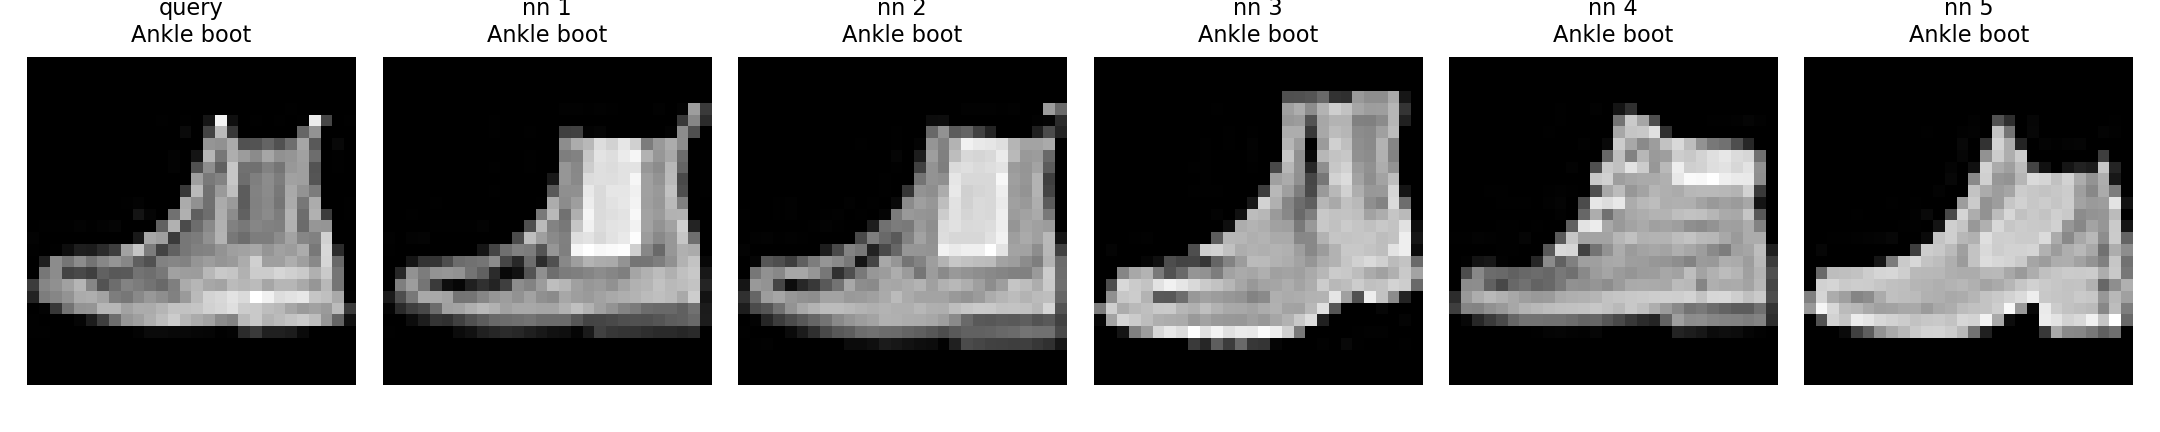
\includegraphics[width=\linewidth]{query_0.png}
  \caption{Query 0}
\end{subfigure}
\hfill
\begin{subfigure}{0.32\linewidth}
  \centering
  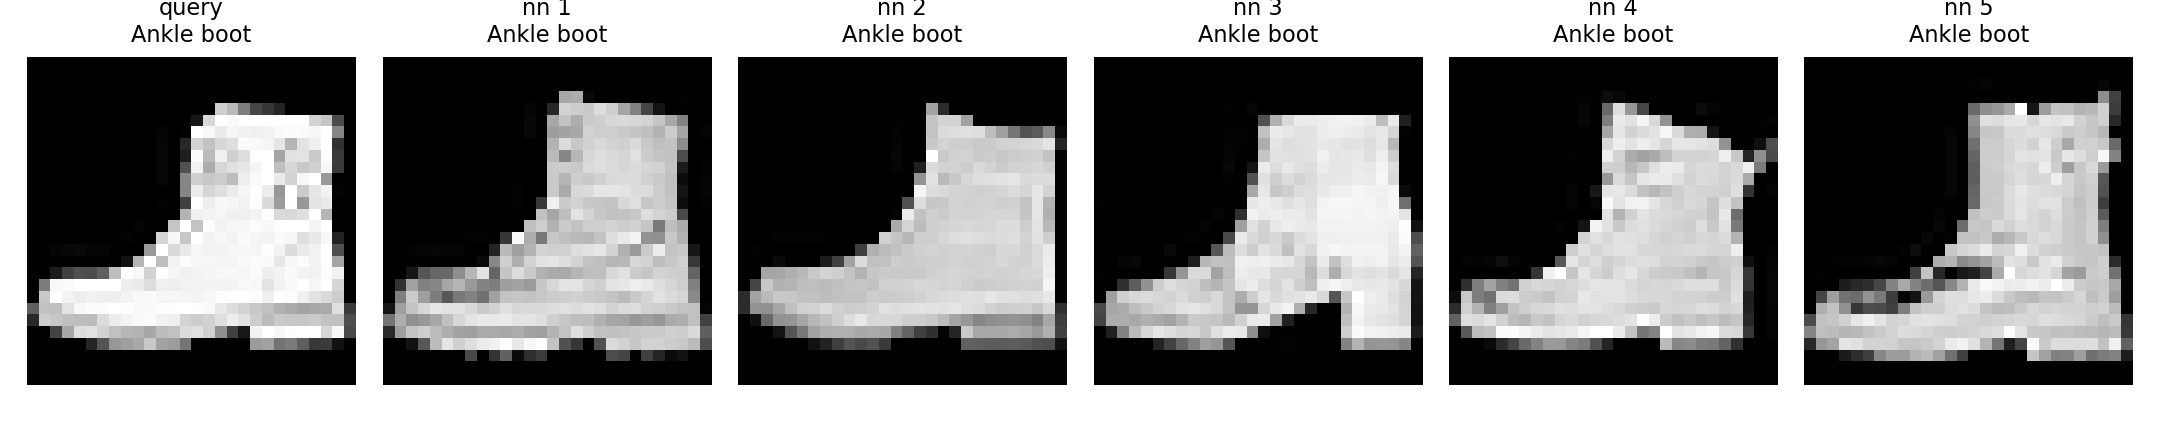
\includegraphics[width=\linewidth]{query_17.png}
  \caption{Query 17}
\end{subfigure}
\hfill
\begin{subfigure}{0.32\linewidth}
  \centering
  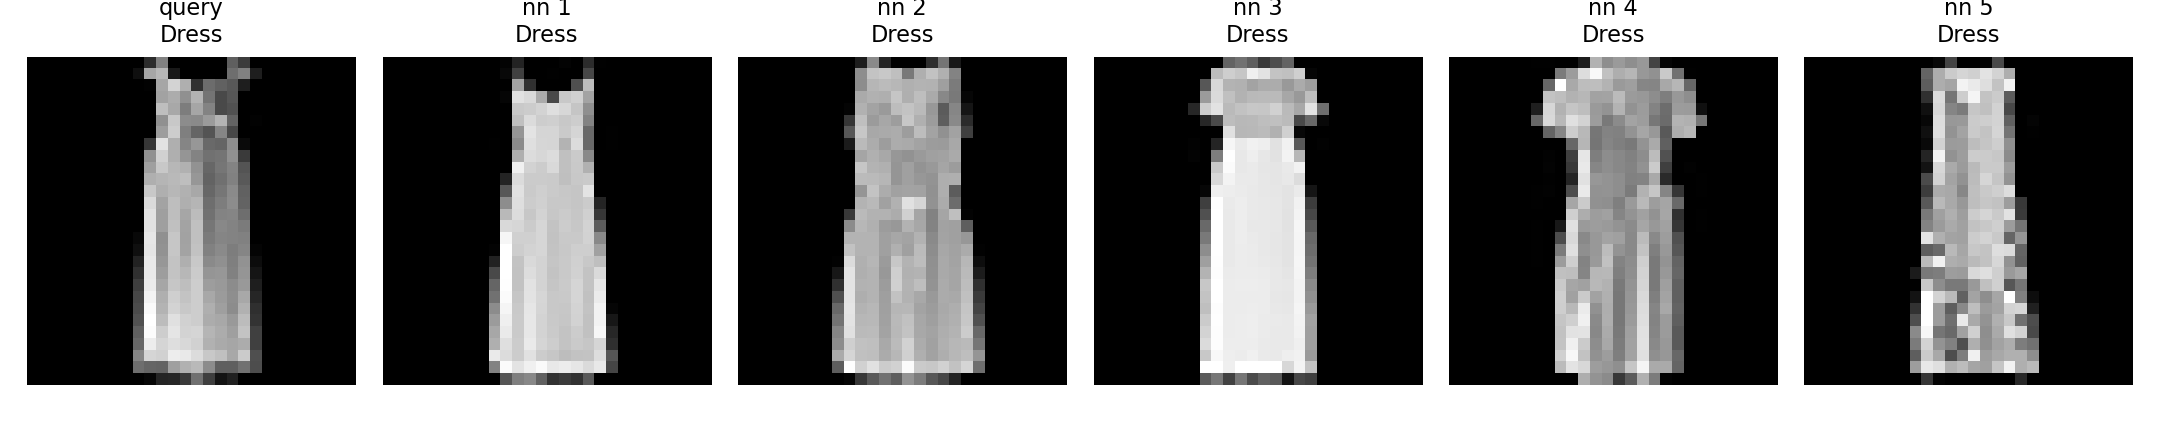
\includegraphics[width=\linewidth]{query_42.png}
  \caption{Query 42}
\end{subfigure}
\caption{Qualitative retrieval examples. Each panel shows a query followed by nearest neighbors.}
\label{fig:retrieval}
\end{figure}

\begin{figure}[H]
\centering
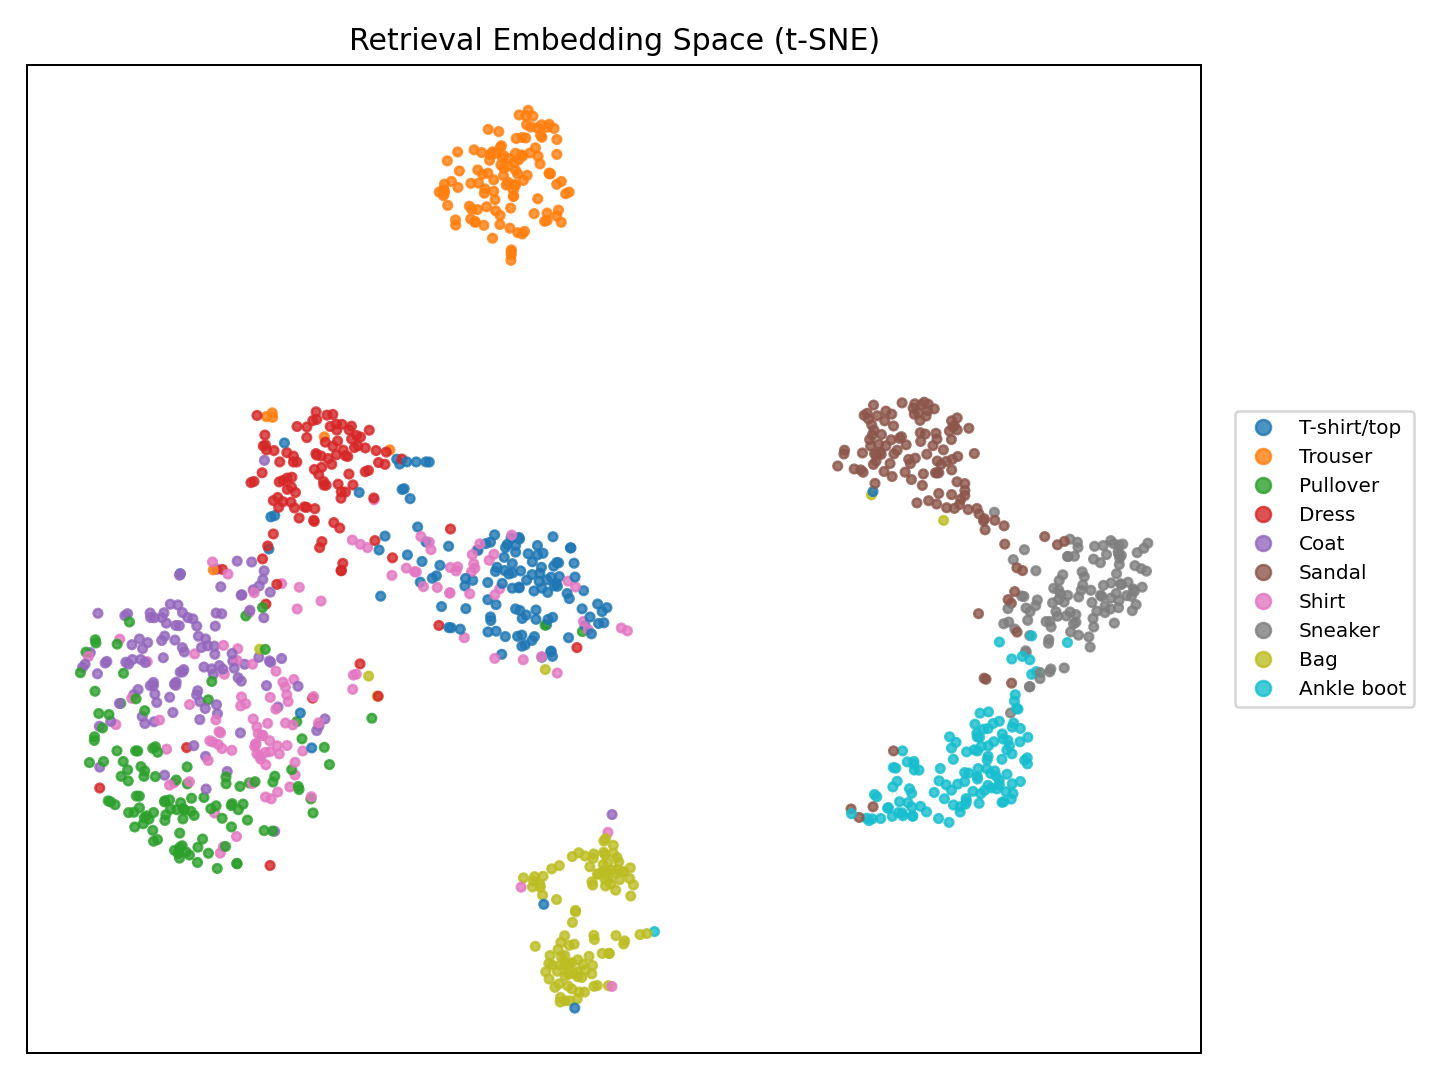
\includegraphics[width=0.66\linewidth]{embedding_tsne.png}
\caption{t-SNE visualization of 1,200 retrieval embeddings, using perplexity 30 and seed 42.}
\label{fig:tsne}
\end{figure}

The class-level results also explain where retrieval is weaker. Bags, trousers, sandals, sneakers, and ankle boots retrieve well, while Shirt is the hardest class (Recall@1 = 0.4975). This is expected because FashionMNIST upper-garment classes such as Shirt, T-shirt/top, Pullover, and Coat are visually close. The full top-1 retrieval confusion matrix is saved with the submitted figures.

\section{Part C: Compression}

Part C keeps the Part B retrieval teacher and compares the two required compression methods: pruning and knowledge distillation. For pruning, I use 40\% global unstructured L1 pruning because it is a simple magnitude-based baseline and directly tests whether small weights can be removed \cite{han2015learning}. For distillation, I train the fixed \model{CompactSeparableCNN} student with relational knowledge distillation (RKD), because the teacher produces embeddings rather than class logits; matching pairwise distances and angles is more relevant for retrieval than matching class probabilities \cite{park2019relational}.

\begin{table}[H]
\centering
\small
\begin{tabular}{lrrrrr}
\toprule
\textbf{Model} & \textbf{Recall@1} & \textbf{Preserved} & \textbf{Params} & \textbf{Nonzero} & \textbf{FLOPs} \\
\midrule
Teacher retrieval model & 0.8295 & 100.0\% & 38,304 & 38,304 & 3,986,624 \\
40\% global L1 pruned teacher & 0.7495 & 90.4\% & 38,304 & 23,456 & 3,986,624 \\
RKD compact student & 0.7890 & 95.1\% & 12,528 & 12,528 & 1,190,528 \\
\bottomrule
\end{tabular}
\caption{Part C compression results.}
\label{tab:partc}
\end{table}

Pruning keeps 90.4\% of teacher Recall@1, but dense FLOPs stay the same because the model is still dense. It would only help on hardware with sparse support. I used unstructured L1 pruning; structured pruning could reduce FLOPs directly, but usually costs more accuracy at the same sparsity.

The distilled student is the better deployment choice here. It keeps 95.1\% of teacher Recall@1 while reducing parameters from 38,304 to 12,528 and dense FLOPs from 3,986,624 to 1,190,528.

\section{Report Questions}

\textbf{Which backbone would I keep after comparing CNN and separable CNN, and why?}
I would keep \model{SeparableCNN}. It has the highest validation macro F1 in Table~\ref{tab:parta}, and it is also much smaller and cheaper than \model{StandardCNN}. This makes it the best Part A checkpoint to reuse in Part B.

\textbf{Did the retrieval model learn meaningful similarity?}
Yes. Recall@1 reaches 0.8295, well above the roughly 10\% random same-class baseline, and Recall@1/5/10 improve over the initialized embedding. mAP is slightly lower, and Shirt is the hardest class because upper-garment items are visually similar.

\textbf{How much performance was preserved after pruning and distillation?}
The 40\% pruned teacher preserves 90.4\% of the teacher Recall@1. The RKD compact student preserves 95.1\%. So both compression methods keep useful retrieval behavior, but distillation preserves more quality and also reduces dense FLOPs.

\textbf{What final model would I deploy, and why?}
I would deploy the RKD compact student. It is smaller, has 3.35$\times$ fewer dense FLOPs than the teacher, and preserves more Recall@1 than the pruned model. I would not choose the pruned model as the default limited-hardware deployment unless sparse operations are supported, because its dense FLOPs are unchanged.

\section{Run Instructions}

The full pipeline can be rerun with:

\begin{verbatim}
python3 -m venv .venv
. .venv/bin/activate
python -m pip install -r requirements.txt
python src/run_project.py
\end{verbatim}

The main outputs are stored in \model{outputs/part\_a/}, \model{outputs/part\_b/}, \model{outputs/part\_c/}, and \model{outputs/figures/}. Local folders such as \model{.venv/}, \model{data/}, and \model{\_\_pycache\_\_/} are not part of the submission.

\bibliographystyle{plain}
\bibliography{references}

\end{document}
